\documentclass[a4paper]{article}
\usepackage{amsfonts}
\usepackage{amsmath}
\usepackage{amssymb}
\usepackage{graphicx}

\newcommand{\dint}{\displaystyle\int}

\begin{document}

\noindent \large Auteur: Rob Willemsen \\
\noindent \large Studierichting: Informatica \\
\noindent \large Oefeningenreeks 5D nr. 4.12 \\

\medskip

\normalsize

$y = x^3$ en $x = 0$ en $y = 1$ \\

Bovengrens: $y = 1$ \\

Ondergrens: $y = x^3$ \\

$S = \dint _0^1 (1 - x^3) dx$ \\

$= \left[x- \dfrac{x^4}{4}\right]_0^1$ \\

$= \left(1 - \dfrac{1}{4}\right) - \left(0 - \dfrac{0^4}{4}\right)$ \\

$= 1 - \dfrac{1}{4} = \dfrac{3}{4}$ \\

\begin{figure}[h]
\centering
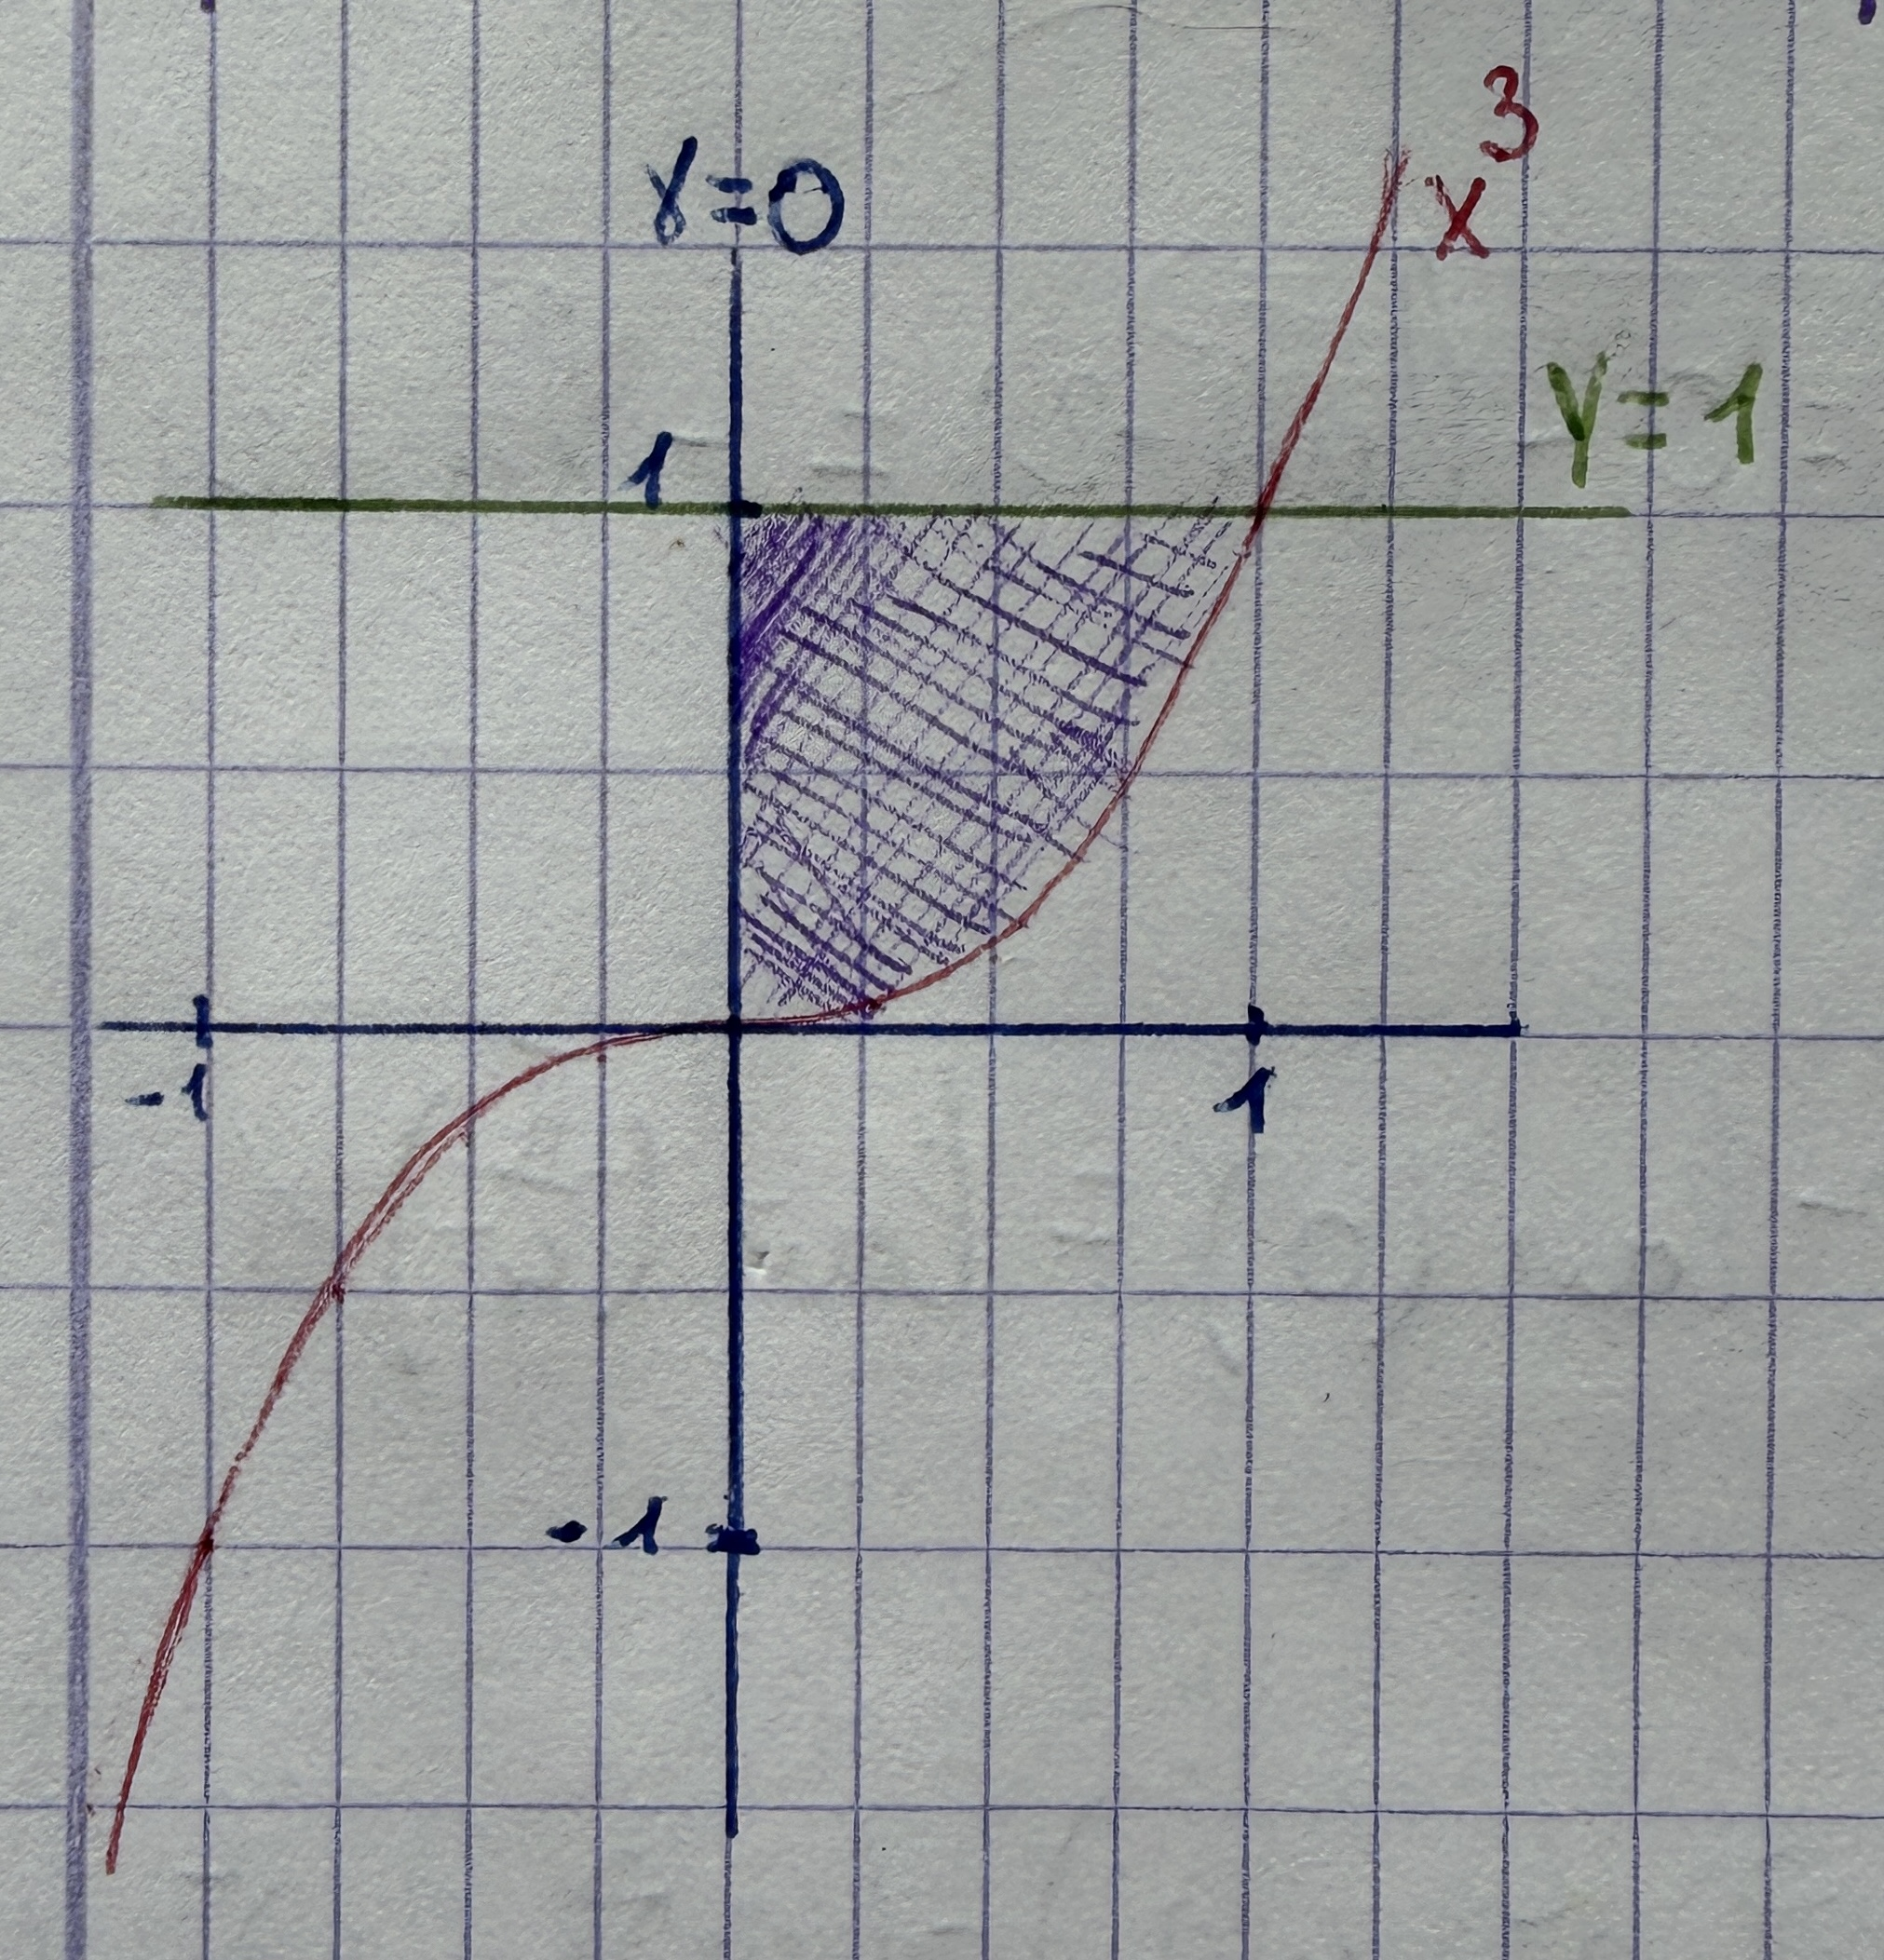
\includegraphics[width=0.5\linewidth]{5D-4.12-rob.willemsen.INF.png}
\end{figure} 

\begin{thebibliography}{999}
%\bibitem{a} Referentie
\end{thebibliography}
\end{document}